\documentclass{article}
\usepackage[margin=25mm]{geometry} % 25 mm margins all around
\usepackage{graphicx} % for pdf figures


\begin{document}



\section*{Fig. 1}
\begin{figure}[ht]
	\centering
	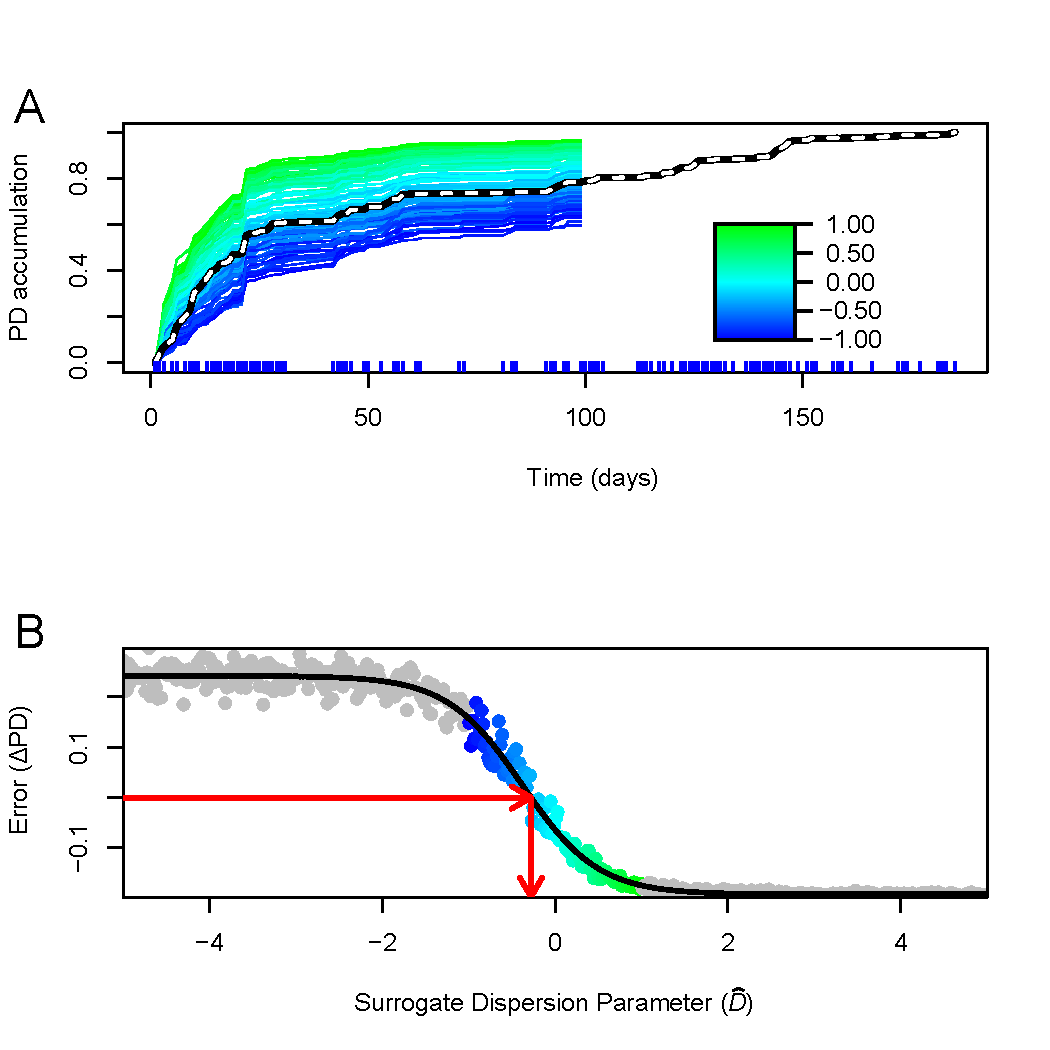
\includegraphics[scale=0.80]{../Fig_1.pdf}
\end{figure}
Phylodiversity accumulation and model fitting in the female feces data set [25]. Plot A shows empirical (dashed) and surrogate phylodiversity accumulation curves. Surrogate curves are colored according to \(\hat{D}\) value (Equation 1). New species that have a previously-detected close relative contribute little phylodiversity and cause slow phylodiversity accumulation (blue). New species that do not have a close relative contribute more phylodiversity and cause faster accumulation (green). The empirical model (dashed) is below the neutral model (teal), signifying underdispersion in the order of first-time species detections. The times of sampling points are shown as vertical blue lines below the X-axis. Curves are rescaled from 0 to 1 in this figure. Plot B shows how empirical and surrogate data are compared to generate an estimate for \(D\). Differences between empirical and surrogate data at time \(m\) are shown on the Y-axis, and the \(\hat{D}\) values used to generate surrogate data sets are shown on the X-axis. Color-coded points correspond to surrogate data sets shown in plot A. Values shown in gray result from using extreme values of \(\hat{D}\), which help the logistic error model (black line) fit to the data, and are not shown in plot A. The red arrows show the process of error minimization, yielding a \(D\) estimate. A figure showing significance testing for these data is available as Fig. S1.
%
\newpage
%
%
\section*{Fig. 2}
\begin{figure}[ht]
	\centering
	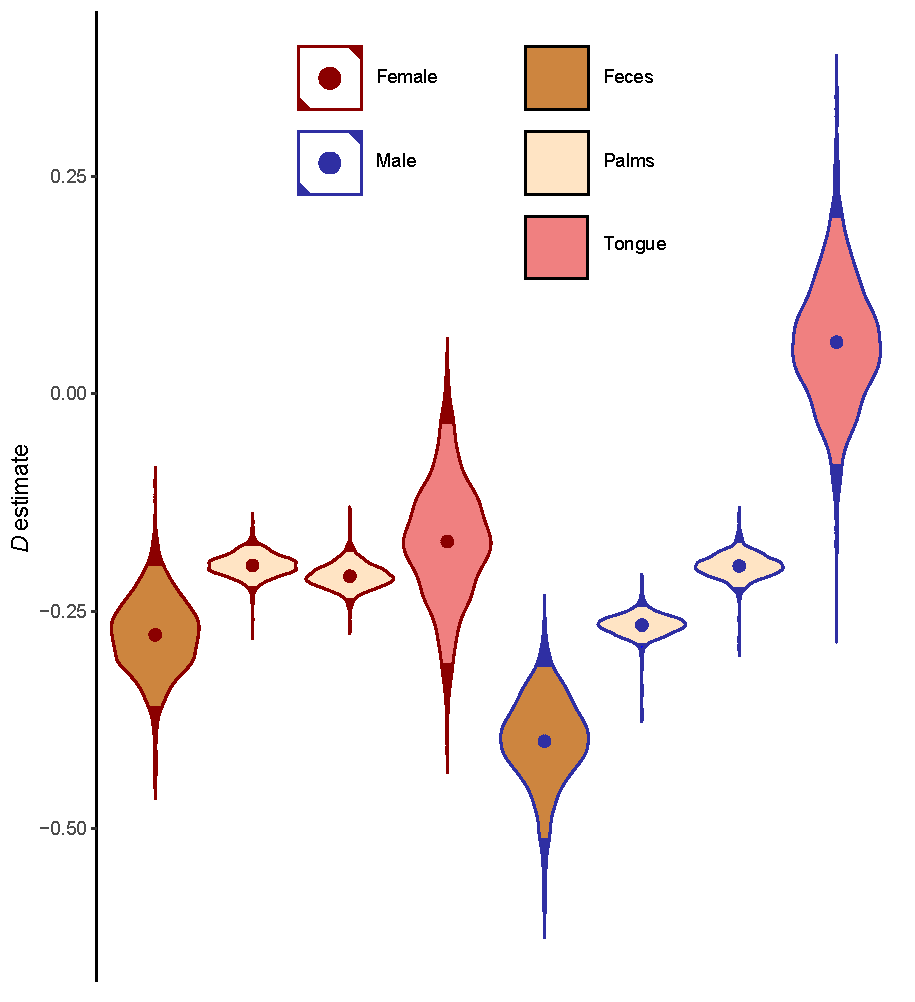
\includegraphics[scale=0.80]{../Fig_2.pdf}
\end{figure}
Dispersion parameter (\(D\)) estimates for "moving pictures" [25] data sets. The subject’s sex is shown as the outline color of each violin, and the body site is shown as fill color. The four body sites for the female subject are shown at left, and the four body sites for the male subject are shown at right. Each violin shows the distribution of \(D\) estimates given by logistic error model bootstraps, and the dots within violins are means. Light-colored portions of violins represent 95\% of bootstraps. The two subjects analyzed show parallel \(D\) estimates, with feces being the lowest, followed by palms which are all similar, followed by tongue communities. For both subjects, tongue patterns were not significantly different than the neutral model.
%
\newpage
%
%
\section*{Fig. 3}
\begin{figure}[ht]
	\centering
	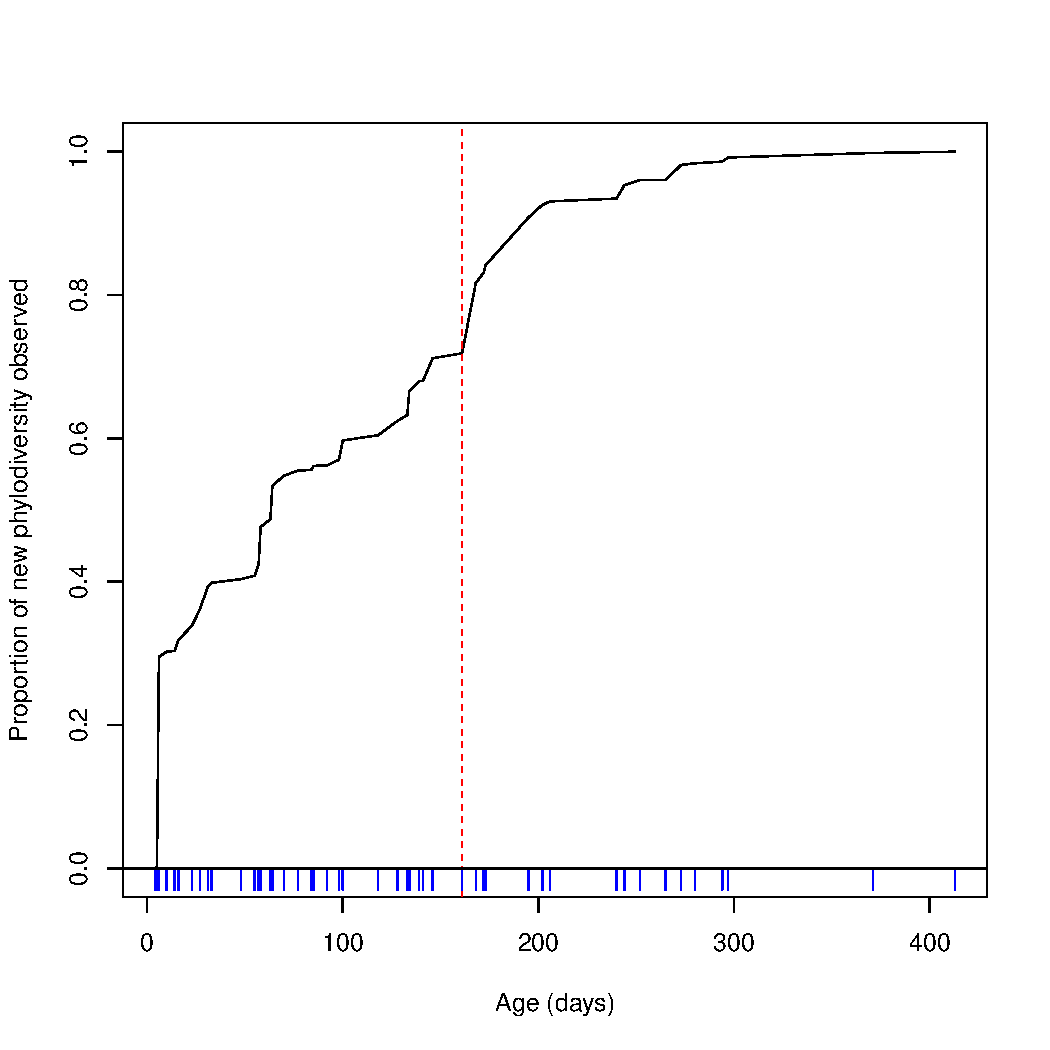
\includegraphics[scale=0.80]{../Fig_3.pdf}
\end{figure}
Empirical phylodiversity accumulation in the infant gut microbiome [26]. Phylodiversity increases sharply after day 161 of the infant’s life, then plateaus. This timing coincides with the day the subject began consuming baby formula. The times of sampling points are shown as vertical blue lines below the X-axis.
%
\newpage
%
%
\section*{Fig. 4}
\begin{figure}[ht]
	\centering
	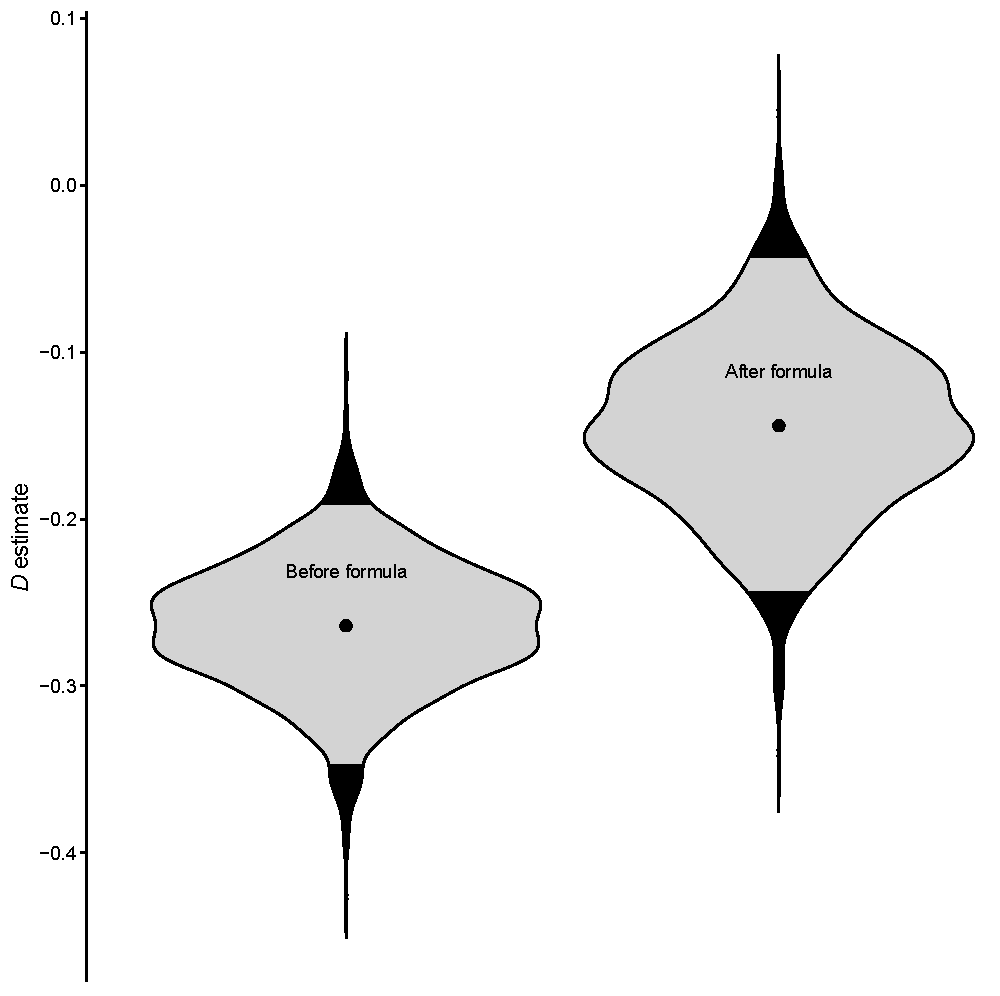
\includegraphics[scale=0.80]{../Fig_4.pdf}
\end{figure}
Dispersion parameter (\(D\)) estimates in the infant gut, pre-formula and during formula use. Formula use began on day 161, thus the first 160 days of the subject's life were analyzed separately. Community assembly was significantly underdispersed in the pre-formula data set, but was not significantly different from the neutral model during formula use (\(P = 0.107\)).
%
\end{document}